\chapter{Descrizione del lavoro}
\label{scenario}
Per comprendere la soluzione proposta e il sistema ideato utilizzeremo un approccio top-down. Partendo da un livello d'astrazione tale in cui emergono solo i requisiti funzionali e il sistema è rappresentato da una \textit{black box}, scenderemo ad un livello che ci permetterà di affinare i requisiti iniziali e mostrare i \textit{sottosistemi} che lo costituiscono. Infine nell'ultimo livello avremo una visione dei \textit{moduli} che compongono i sottosistemi e che sono stati realizzati nel contesto di questa tesi.
\begin{figure}[H]
	\centering
	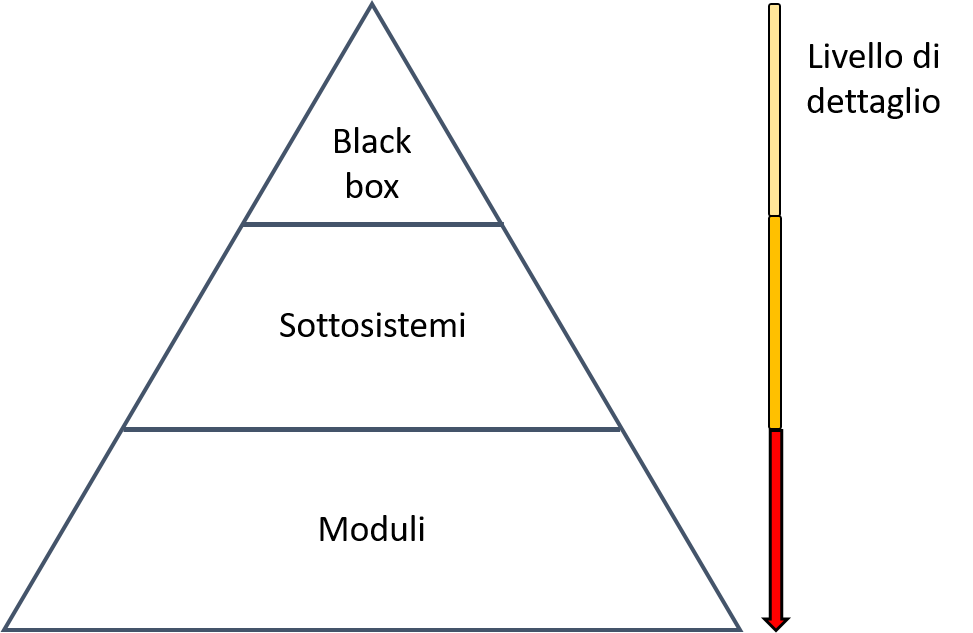
\includegraphics[scale=0.4]{DescrizioneDelSistema/livelli_astrazione.png}
	\caption{Rappresentazione dei livelli d'astrazione utilizzati per descrivere il sistema }
	\label{fig:livelliAstrazione}
\end{figure}
\newpage

\section{Livello black box}
Considerando il sistema in questione come una black box (Fig.\ref{fig:requisitiFunzionali}) e l'infrastruttura di rete in modo astratto, i due macro-requisiti funzionali  sono rispettivamente:
\begin{itemize}
	\item \textbf{R1}: Geolocalizzare l'operatore
	\item \textbf{R2}: Trasmettere messaggi predefiniti come stato della vittima e codici d'emergenza.
\end{itemize}
\begin{figure}[H]
	\centering
	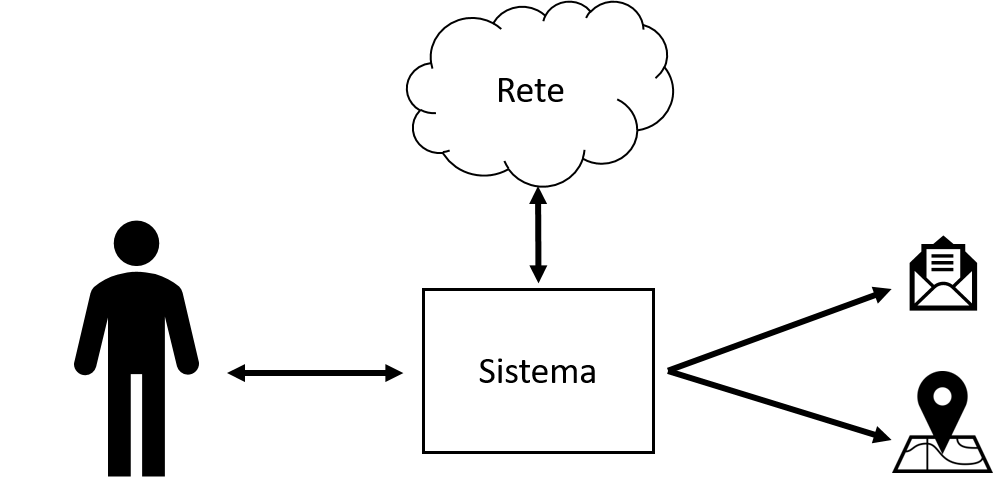
\includegraphics[scale=0.3]{DescrizioneDelSistema/requisitiSistema.png}
	\caption{Rappresentazione del sistema come black box }
	\label{fig:requisitiFunzionali}
\end{figure}
Nelle fasi primordiali del progetto, si è scelto di allocare la maggior parte delle risorse lavorative nel completamento di \textbf{R1} lasciando ad una fase successiva lo sviluppo di \textbf{R2}, per questo motivo d'ora in avanti considereremo come unico requisito la geolocalizzazione dell'operatore. \textit{R1} può essere suddiviso in due requisiti più specifici:
\begin{itemize}
	\item \textbf{R1.1}: Determinare la posizione di un operatore all'interno della rete
	\item \textbf{R1.2}: Identificare il cammino minimo da un nodo ad un altro
\end{itemize}
Quest'ultimo rappresenta sia la possibilità da parte dell'operatore di eseguire il percorso all'inverso, sia la possibilità che venga raggiunto da una squadra di supporto. A questo punto possiamo scendere al livello d'astrazione successivo (\ref{fig:livelliAstrazione}).
\newpage 


\section{Livello sottosistemi}
\label{livello_sottosistemi}
Come già accennato nell'introduzione, la rete verrà costruita dinamicamente da un'esploratore e man mano che egli avanza verrà ampliata aggiungendo nuovi nodi.
Realizzare una rete del genere introduce numerose problematiche, alcune strettamente legate alla tecnologia utilizzata (vedi cap.\ref{tecnologie}) altre alle caratteristiche richieste.\\
Nello specifico la problematica sulla quale il lavoro di questi tesi si è concentrato è la progettazione e lo sviluppo dei sottosistemi destinati alla georeferenziazione della rete, ovvero l'attribuzione dell'informazione riguardante la dislocazione geografica dei nodi all'interno della rete.\\
In questo contesto i sottosistemi individuati nella fase di progettazione sono rappresentati dalla seguente figura: 
\begin{figure}[H]
	\centering
	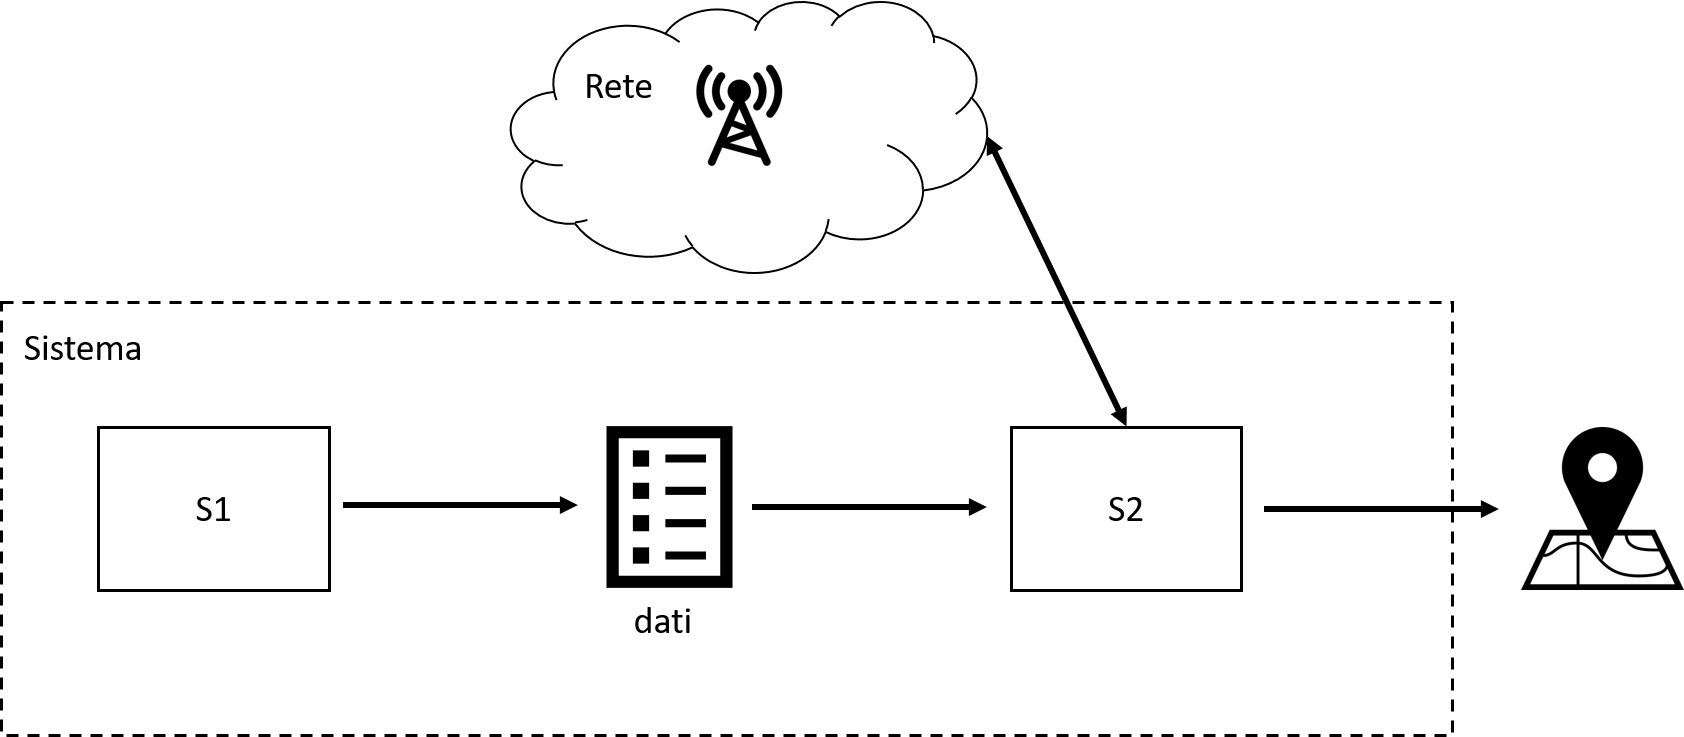
\includegraphics[scale=0.3]{DescrizioneDelSistema/sistema_liv1.png}
	\caption{Rappresentazione del sistema in sottosistemi }
	\label{fig:sistema_liv1}
\end{figure}

Ognuno dei quali con la propria responsabilità:
\begin{itemize}
	\item \textbf{S1}: ha il compito di ricavare tramite la rete e altri sensori i dati necessari
	\item \textbf{App}: ha il compito di ricevere i dati da S1, elaborarli e infine fornire la posizione del nuovo nodo rispetto alla rete
\end{itemize}

La soluzione al problema si costruisce per iterazione georeferenziando i singoli nodi nel momento in cui vengono aggiunti dall'operatore. Con riferimento all'esempio illustrato precedentemente (vedi Fig.\ref{fig:step1}- Fig.\ref{fig:step6}) consideriamo lo step 2.\\
Per ipotesi supponiamo che il primo nodo sia già georeferenziato, nel momento in cui l'operatore risulti essere al limite della line-of-sight e/o della distanza di sicurezza (20 mt) piazzerà il secondo nodo. Per georeferenziarlo (rispetto al primo) abbiamo bisogno di due informazioni fondamentali:
\begin{itemize}
	\item La distanza tra i due nodi
	\item L'angolo tra i due nodi
\end{itemize} 
Per mantenere il livello d'astrazione attuale ci basta sapere che le caratteristiche della tecnologia utilizzata nell'implementazione della rete, fa si che le singole celle abbiano un raggio d'azione all'interno del quale il sottosistema \textit{S1} può calcolare la distanza tra l'operatore e il centro della cella di appartenenza.\\
Tale informazione non è però sufficiente, infatti ci sono infiniti punti sulla circonferenza con centro nel primo nodo e raggio pari alla distanza. Per poter georeferenziare in modo univoco il secondo nodo abbiamo bisogno di trovare anche l'angolo in riferimento al primo nodo, tale compito non è banale e tanto meno le metodologie univoche e perfette.\\
La figura seguente rappresenta un tentativo di georeferenziare il secondo nodo utilizzando soltanto la distanza tra i due nodi.
\begin{figure}[H]
	\centering
	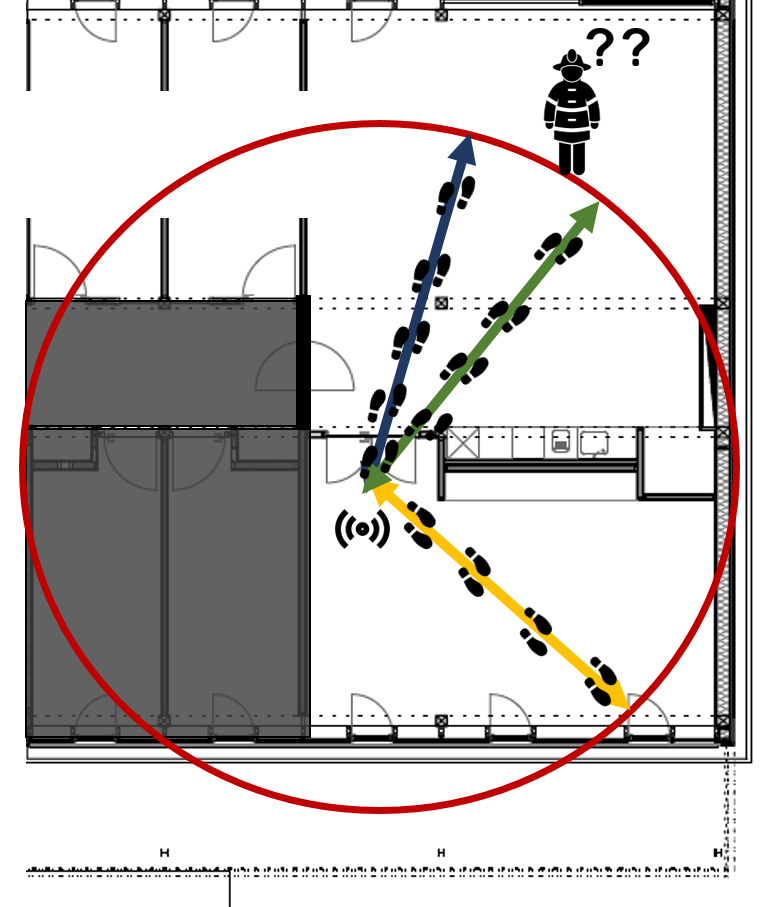
\includegraphics[scale=0.35]{DescrizioneDelSistema/ambiguitDistanza.png}
	\caption{Ambiguità nella georeferenziazione di un secondo nodo utilizzando soltanto la distanza dal precedente }
	\label{fig:ambiguitDistanz}
\end{figure}
Nell'esempio appena proposto, abbiamo mostrato solo tre delle possibili infinite posizioni del secondo nodo. Assumiamo che il punto corretto sia l'intersezione tra il vettore in blu e la circonferenza. In tal caso un'ambiguità con il vettore in verde potrebbe essere accettata in quanto si discosta di pochi metri dalla reale posizione, ben diversa sarebbe un'ambiguità con il vettore in giallo che renderebbe l'informazione del tutto errata e il sistema disinformante.\\
Per il momento ci basta sapere che l'algoritmo utilizzato nel contesto di questa tesi (vedi cap.\ref{data_fusion}), esegue un campionamento durante il tragitto tra un nodo e l'altro combinando i dati inerenti alla distanza dell'operatore con quelli relativi agli angoli lungo il percorso.
Nel prossimo paragrafo ci porteremo al livello d'astrazione più basso della nostra piramide (vedi \ref{fig:livelliAstrazione}) dettagliando i moduli che compongono i due sottosistemi e illustrando come questi intendono risolvere il problema di georeferenziazione appena esposto. \newpage


\section{Livello moduli}

Prima di "aprire" i due sottosistemi è bene specificare che utilizzeremo il termine \textit{modulo} per riferirci sia a componenti hardware che software. Questo abuso di notazione ci permetterà di mostrare con un unico livello d'astrazione tutti i moduli progettati e realizzati al fine di risolvere il problema della georeferenziazione dei nodi.
\begin{figure}[H]  
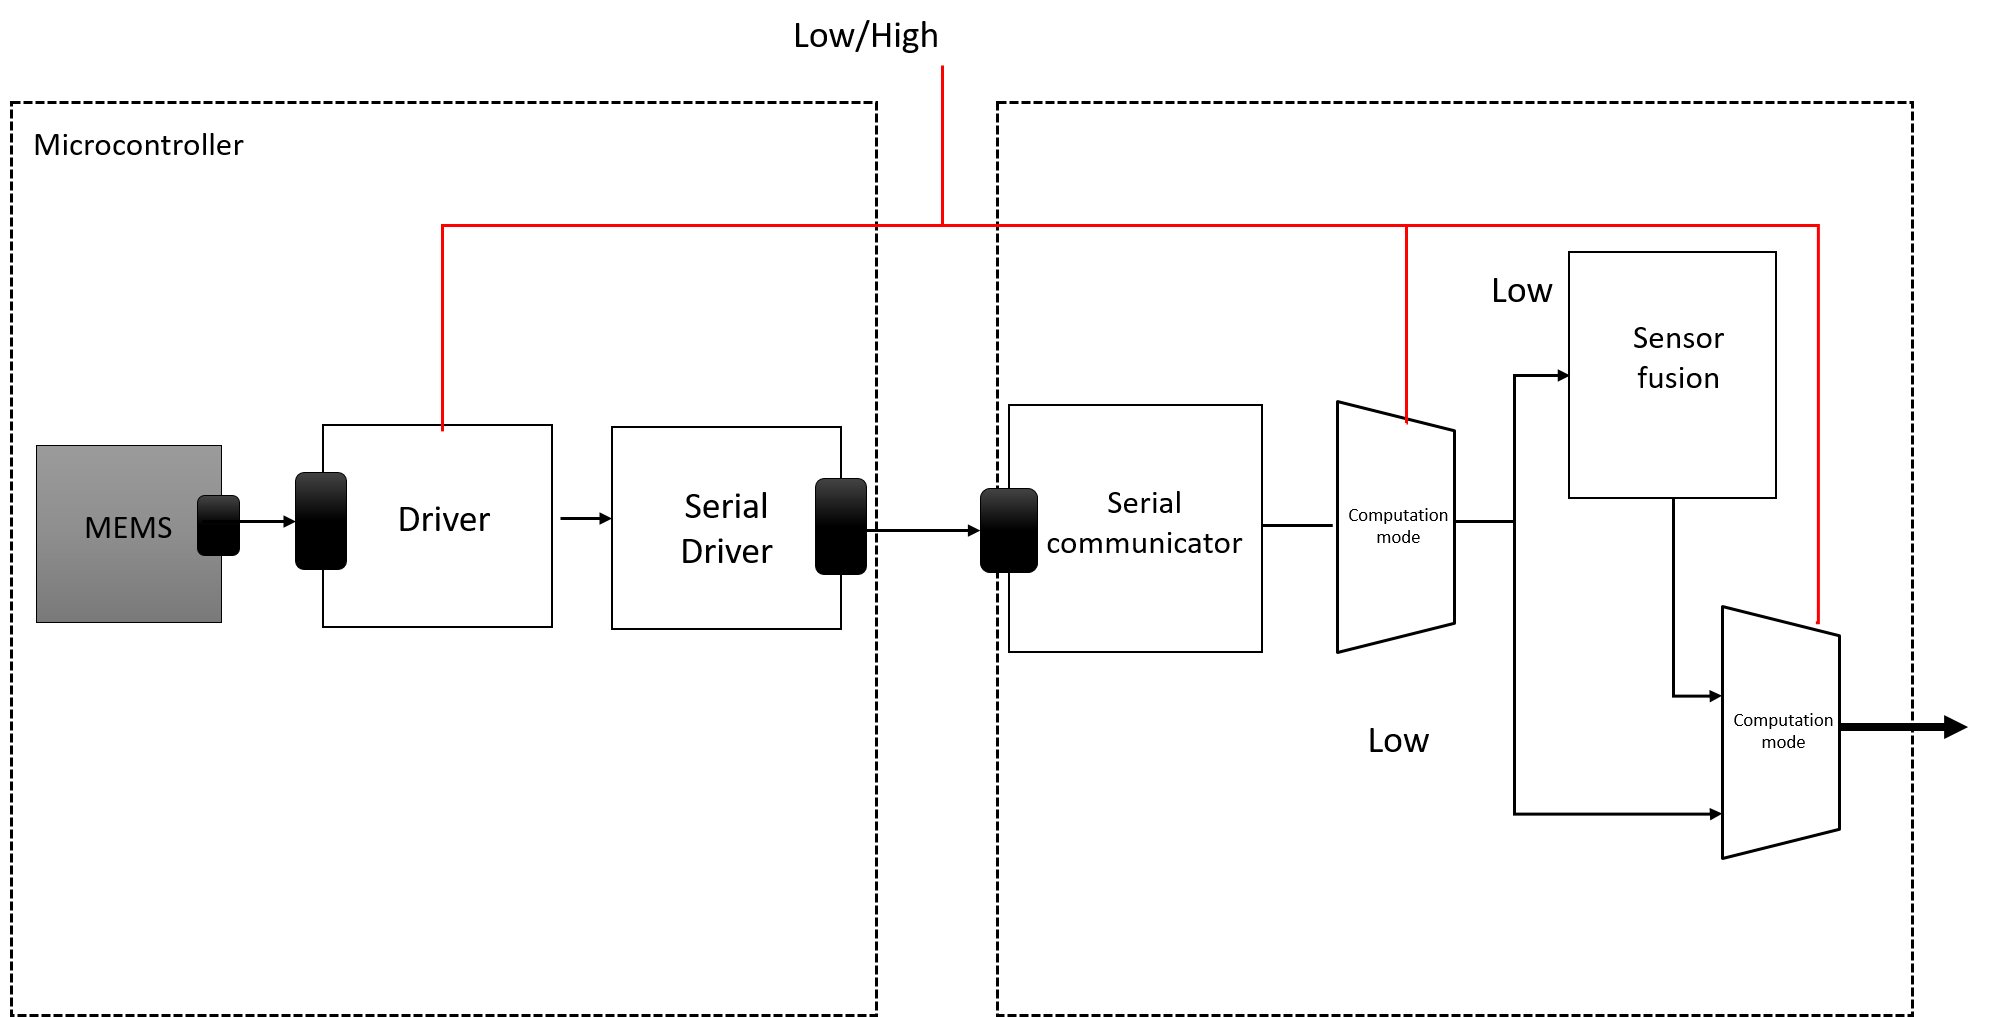
\includegraphics[scale=0.3 ]{DescrizioneDelSistema/sistema_liv2.png}
\caption{Rappresentazione dei sottosistemi in moduli}
\label{fig:sistema_liv2}
\end{figure}
Per esplicare al meglio i compiti dei singoli moduli e mantenere l'attuale livello d'astrazione, fermo restando che tutti i dettagli tecnici verranno forniti nei capitoli successivi, mostreremo il flusso di dati generato in uno qualsiasi degli intervalli di campionamento lungo il tragitto dell'operatore tra un nodo e l'altro.\\ 
Il flusso inizia nel momento in cui il \textit{driver} acquisisce le informazioni dai moduli \textit{MEMS} e \textit{UWB} riguardanti la distanza, la velocità angolare e l'accelerazione lineare dell'operatore. Come mostrato dalla figura seguente. 
\begin{figure}[H] 
	\centering 
	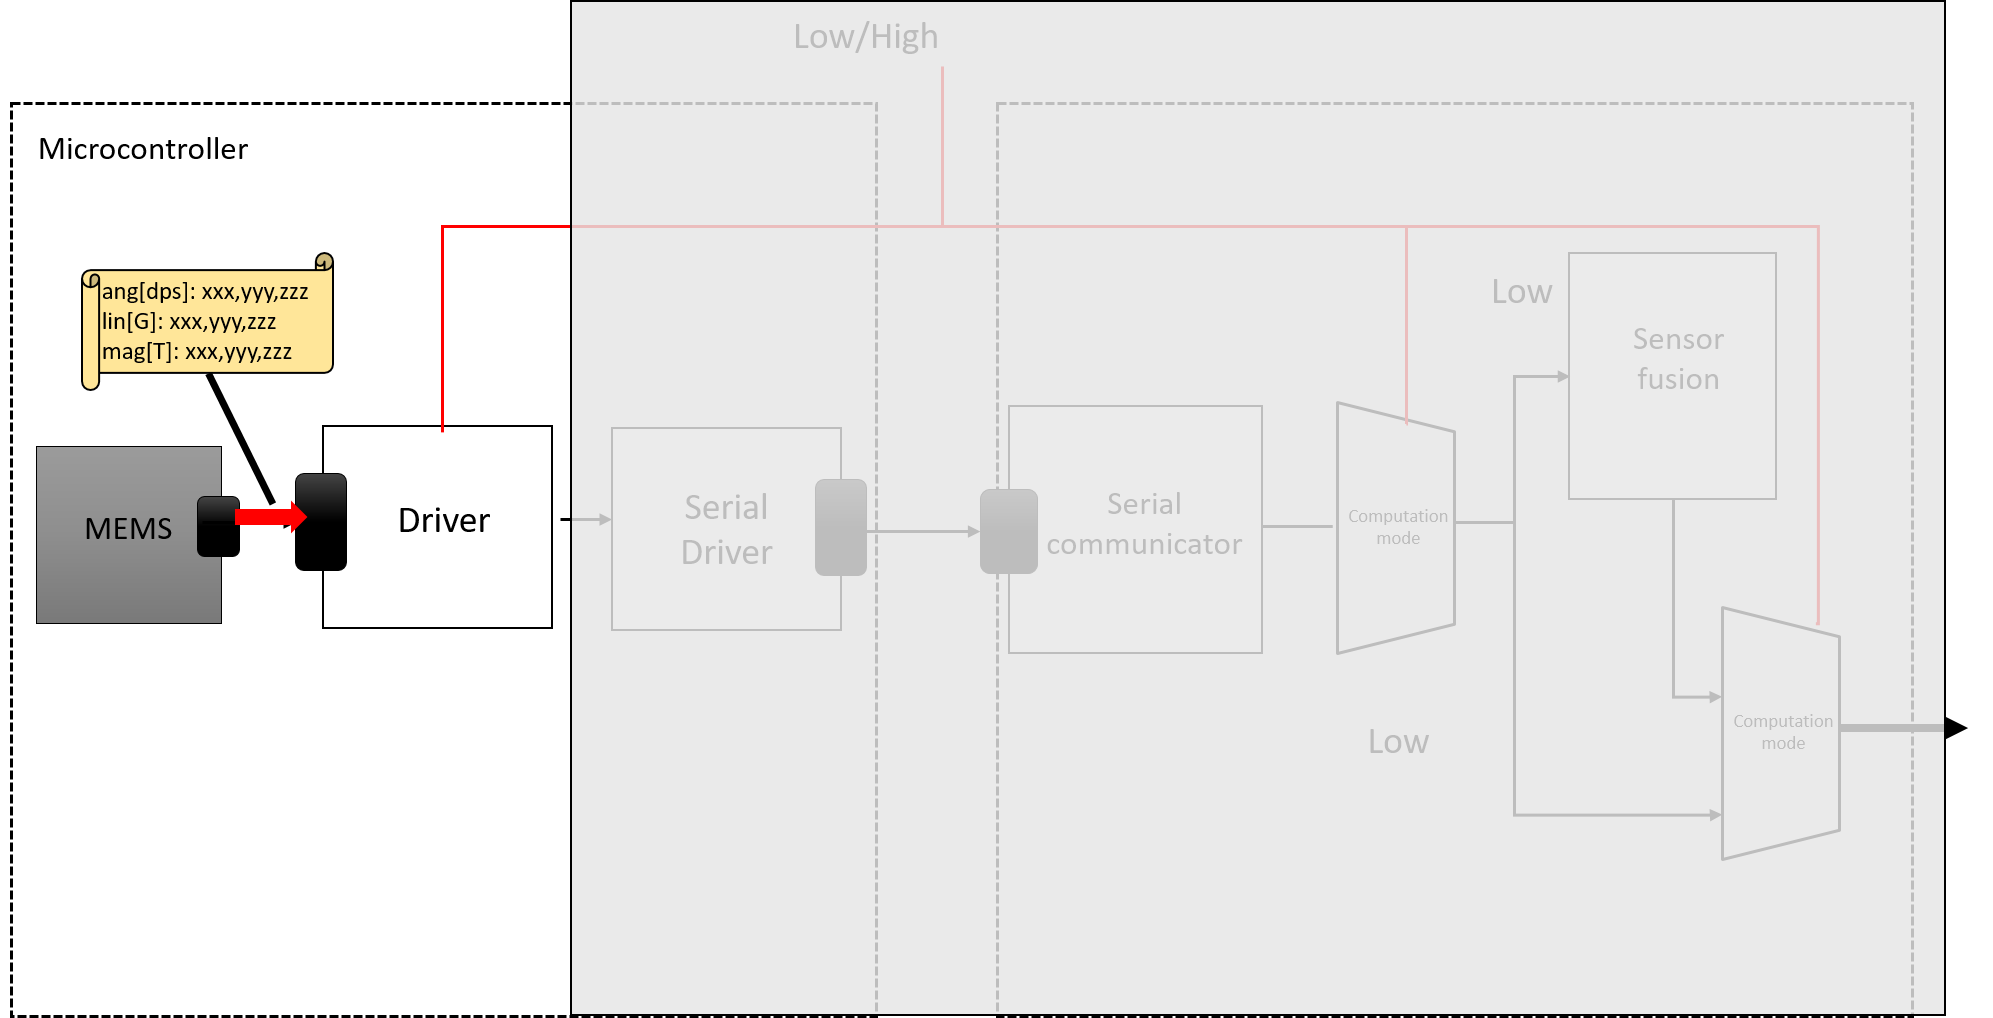
\includegraphics[scale=0.25 ]{DescrizioneDelSistema/flusso1.png}
	\caption{Rappresentazione del flusso di dati tra i moduli dei sottosistemi, step 1}
	\label{fig:flusso1}
\end{figure}
I dati acquisiti sono "grezzi" e devono essere elaborati (vedi cap.\ref{rumore}). Quando e da chi questa computazione verrà eseguita durante il flusso, viene stabilito attraverso il comando Low/High. Da questo ne consegue anche la modalità di funzionamento del driver in:
\begin{itemize}
	\item \textbf{HCM}: High Computation mode, i dati vengono elaborati dal microcontrollore
	\item \textbf{LCM}: Low Computation mode, i dati verranno elaborati in seguito dal sottosistema \textit{App} 
\end{itemize}
La scelta tra quale di queste due modalità utilizzare verrà motivata nel capitolo riguardante l'analisi dei risultati (cap.\ref{elaborazione}), per il momento ipotizziamo di settare la linea di comando al valore "Low" e quindi di utilizzare il driver in \textit{LCM}. Con queste impostazioni i dati grezzi vengono impacchettati ed etichettati con un timestep relativo, prima di essere inviati dal modulo \textit{Serial driver} e ricevuti dal sottosistema \textit{App} mediante il modulo \textit{Serial communicator}, quest'ultimo non farà altro che inoltrarli all'ingresso del multiplexer \textit{Computation mode} come mostrato in figura:
\begin{figure}[H]  
	\centering 
	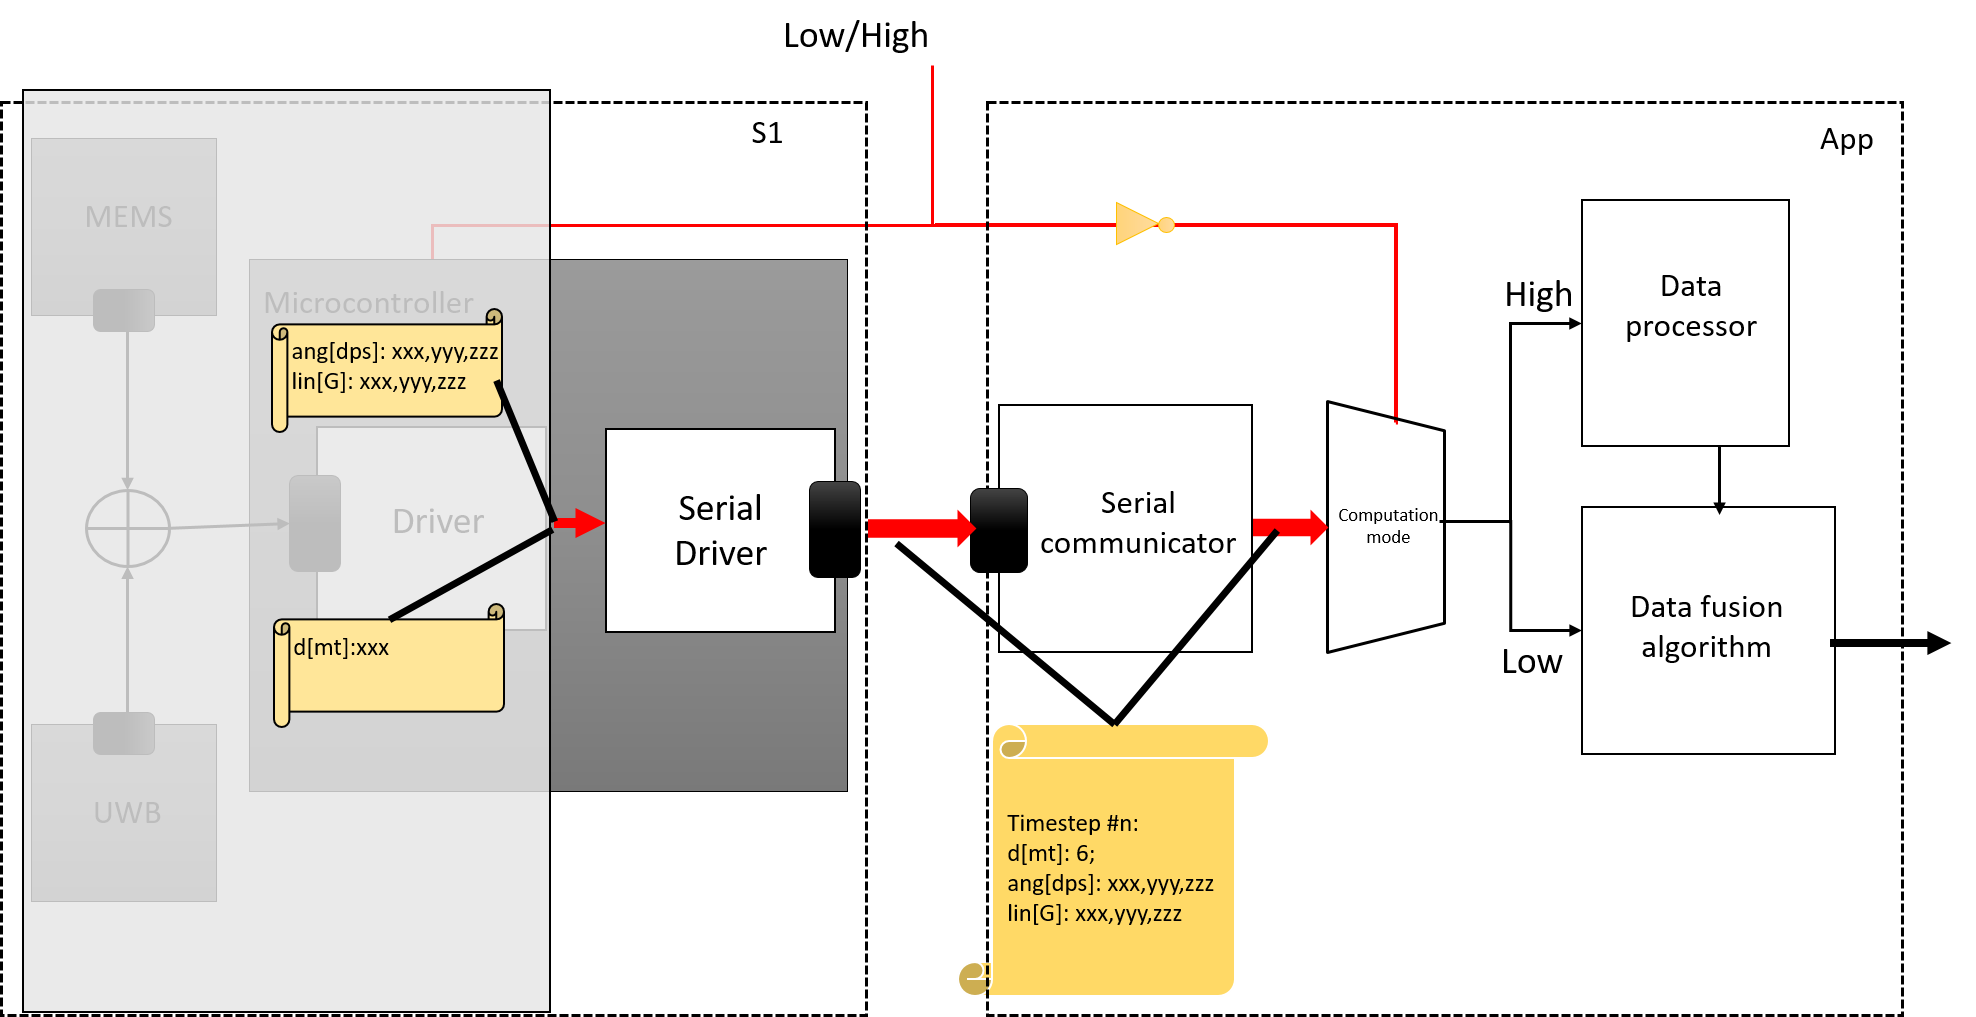
\includegraphics[scale=0.25 ]{DescrizioneDelSistema/flusso2.png}
	\caption{Rappresentazione del flusso di dati tra i moduli dei sottosistemi, step 2}
	\label{fig:flusso2}
\end{figure}
Poiché per ipotesi abbiamo scelto di settare la linea di comando sul valore \textbf{Low}, la sua negazione sul ramo del sottosistema \textit{App} fa si che il multiplexer devii il flusso di dati verso il modulo \textit{Data processor} come mostrato in figura:
 \begin{figure}[H]  
 	\centering 
 	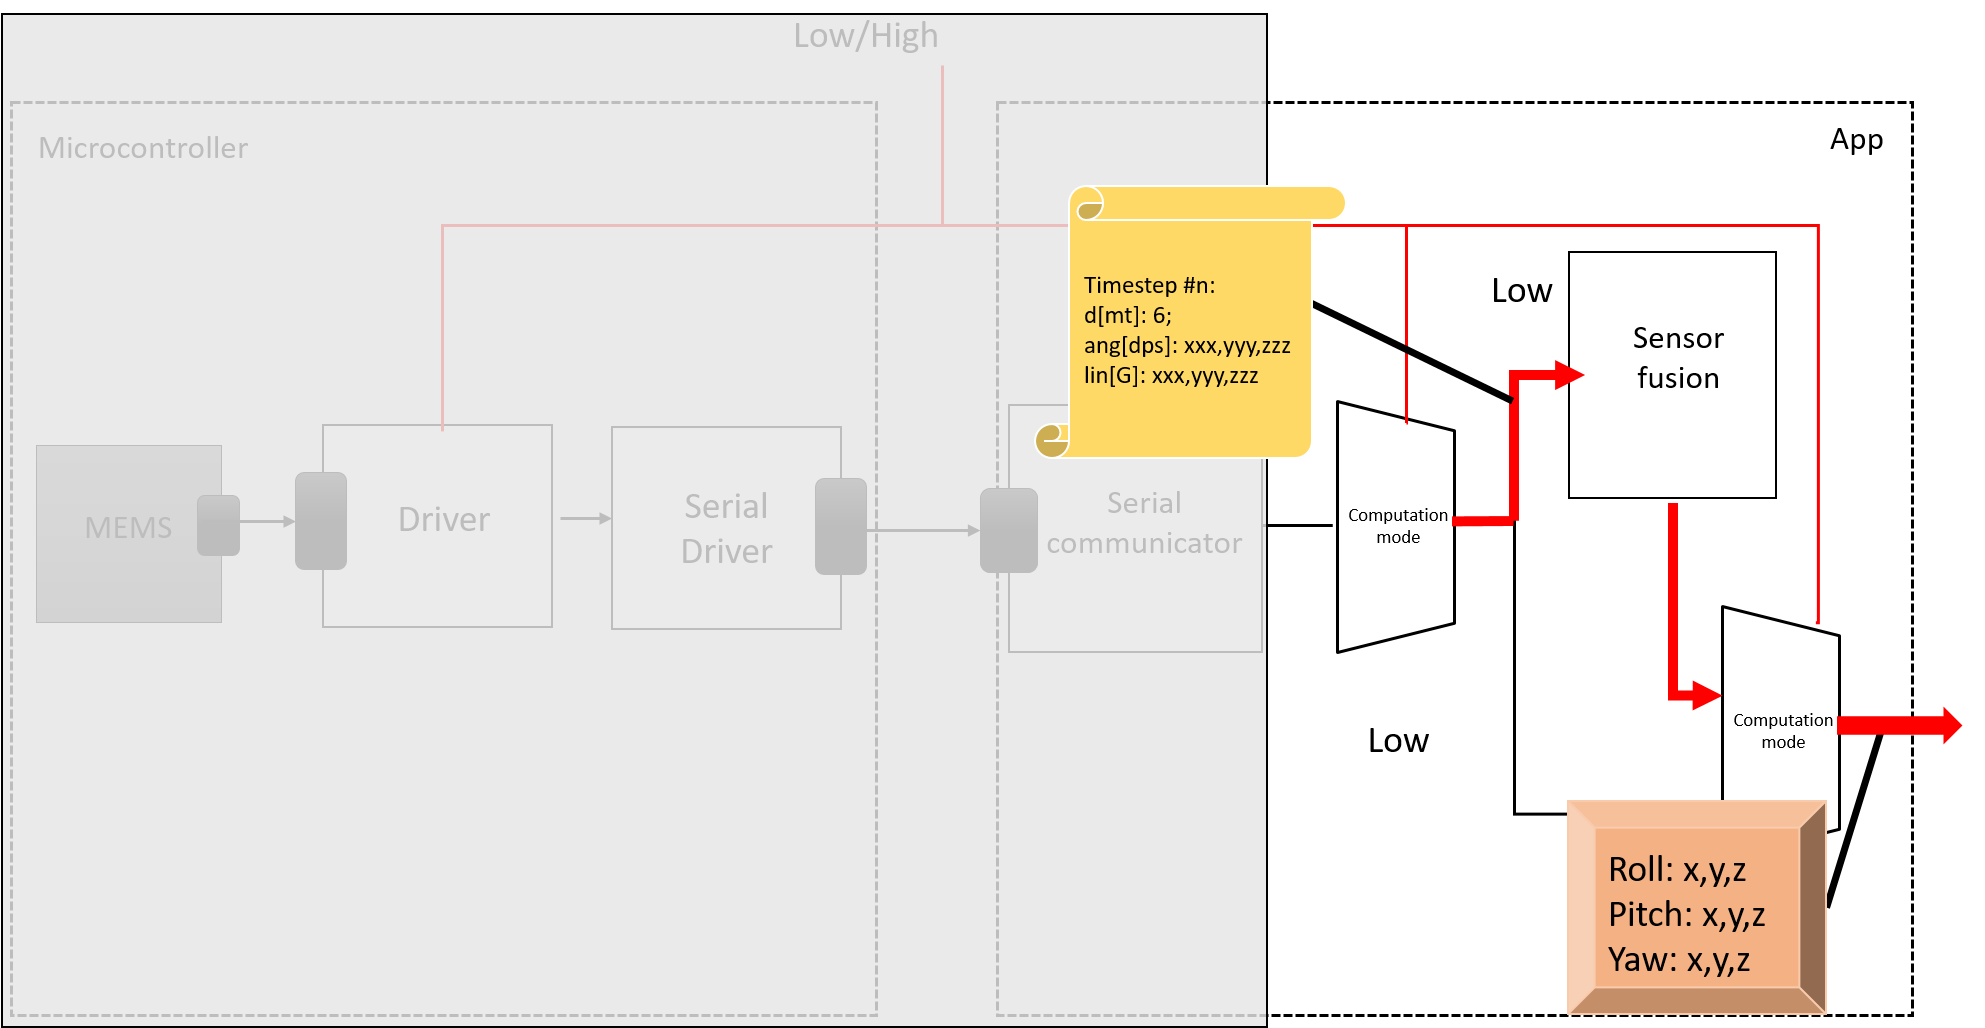
\includegraphics[scale=0.25 ]{DescrizioneDelSistema/flusso3.png}
 	\caption{Rappresentazione del flusso di dati tra i moduli dei sottosistemi, step 3}
 	\label{fig:flusso3}
 \end{figure}
\newpage
A questo punto il modulo \textit{Data processor} elabora i dati grezzi (vedi cap.\ref{elaborazione}) fornendo in uscita le seguenti informazioni:
\begin{itemize}
	\item \textbf{d}: la distanza in metri tra il centro della cella e l'operatore
	\item \textbf{acc}: l'accelerazione lineare dell'operatore lungo gli assi X,Y e Z
	\item \textbf{rot}: i quaternioni di rotazione dell'operatore
\end{itemize}
Infine questi dati verranno usati come input dal modulo \textit{Data fusion algorithm} (vedi \ref{data_fusion}) che provvederà, una volta terminato il tragitto da parte dell'operatore, a determinare l'angolo del nuovo nodo rispetto al precedente e quindi a risolvere il problema di georeferenziazione emerso precedentemente (vedi \ref{livello_sottosistemi}).
 \begin{figure}[H]  
	\centering 
	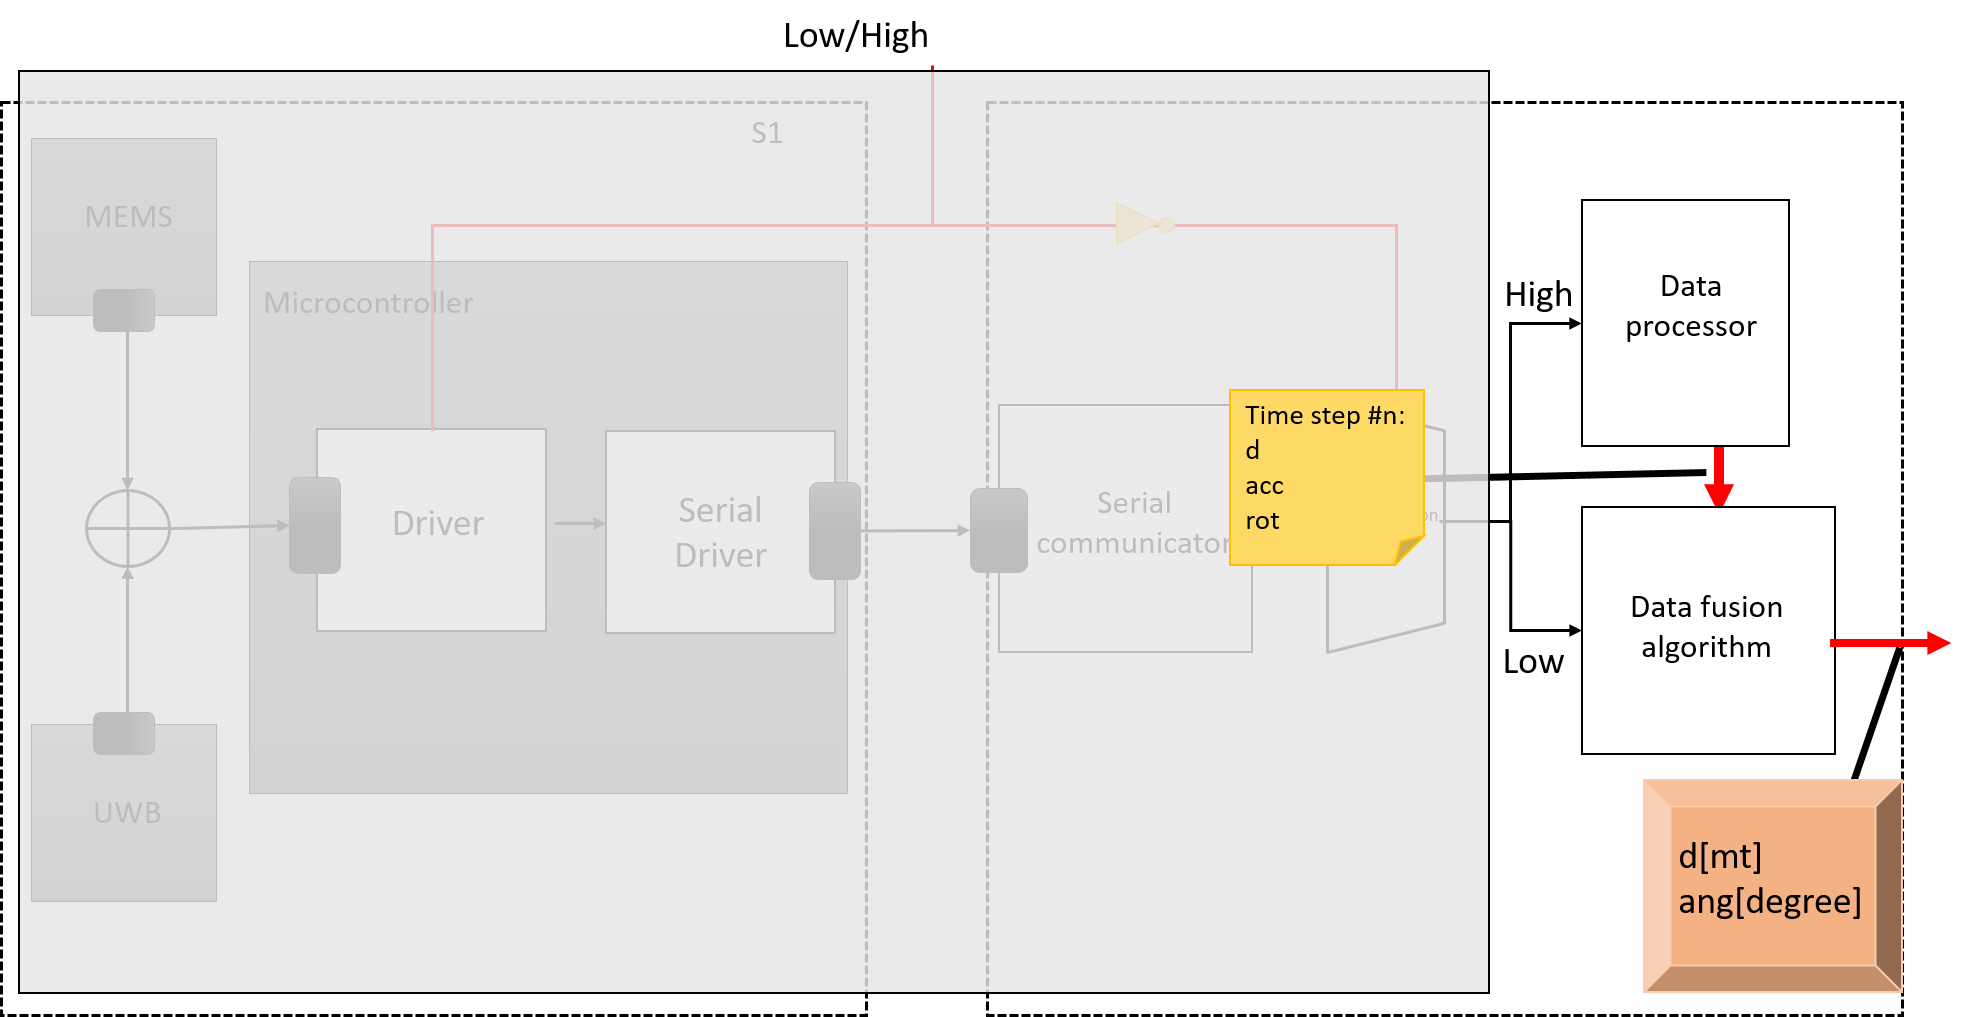
\includegraphics[scale=0.25 ]{DescrizioneDelSistema/flusso4.png}
	\caption{Rappresentazione del flusso di dati tra i moduli dei sottosistemi, step 4}
	\label{fig:flusso4}
\end{figure}